\documentclass[a4paper,10pt]{article}

% Fancy maths stuff
\usepackage{amsmath, amsthm, amssymb}
%\usepackage{fullpage}

% Algorithm typesetting environments
\usepackage{algorithm}
\usepackage{algorithmic}

% Multiline tables
\usepackage{array}
\usepackage{booktabs}

% Trees
\usepackage{qtree}

% Images
\usepackage{graphicx}

\begin{document}

% TITELPAGINA

\begin{titlepage}
\begin{center}

\vspace{2.5cm}

% [CHANGE] The title of your thesis. If your thesis has a subtitle, then this
% should appear right below the main title, in a smaller font.
\begin{Huge}
Performance Rendering using Structure Level Expression
\end{Huge}

\vspace{1.5cm}

% [CHANGE] Your full name. In case of multiple names, you can include their
% initials as well, e.g. "Jan G.J. van der Wegge".
Bastiaan J. van der Weij\\
% [CHANGE] Your student ID, as this has been assigned to you by the UvA
% administration.
5922151

\vspace{1.5cm}

% [DO NOT CHANGE]
Bachelor thesis\\
% [CHANGE] Whether your Bachelor thesis is 6 ECTS (regular) or 9 ECTS (Honours
% programme).
Credits: 15 EC

\vspace{0.5cm}

% [DO NOT CHANGE] The name of the educational programme.
Bachelor Opleiding Kunstmatige Intelligentie

\vspace{0.25cm}

% [DO NOT CHANGE] The addess of the educational programme.
University of Amsterdam\\
Faculty of Science\\
Science Park 904\\
1098 XH Amsterdam

\vspace{4cm}

\emph{Supervisor}\\
% [CHANGE] The name of your supervisor. Include the titles of your supervisor,
% as well as the initials for *all* of his/her first names.
Prof. dr. ir. R.J.H. Scha

\vspace{0.25cm}

% [CHANGE] The address of the institute at which your supervisor is working.
% Be sure to include (1) institute (is appropriate), (2) faculty (if
% appropriate), (3) organisation name, (4) organisation address (2 lines).
Institute for Language and Logic\\
Faculty of Science\\
University of Amsterdam\\
Science Park 904\\
1098 XH  Amsterdam

\vspace{1.5cm}

% [CHANGE] The date at which you will finalize and submit your thesis.
June 24th, 2010

\end{center}

\end{titlepage}



\begin{abstract}
Both machine learning and rule based techniques have been extensively applied to performance rendering. However, relatively few systems make explicit use of machine learning combined with musical structure. Systems that use machine learning usually learn expression at note level. This paper introduces a performance rendering system that learns expression exclusively at a structural level. The system can be seen as complementary to systems that learn expression at note level. 

%Musical structure is extracted automatically. A dataset containing performances aligned to scores is then used to learn how structure relates to expression. A hidden markov model is used to model this relation. Finally, the system can be applied to a a new score to produce an expressive performance. 


%This paper introduces a system for expressively performing transcribed music (scores) using statistical learning from a dataset. The dataset that is used contains performances aligned to the corresponding score. Expression is considered to be the way in which the performance deviates from the score. Expressive actions are predicted from links found between musical structure and expression. Previous expressive actions are also incorporated in the predictions. Musical structure will be automatically extracted from the scores using a set of formal rules that assign a hierarchical grouping structure to the music. To system will be able to deal with polyphonic music by splitting the scores into melody and harmony.

{\bf Keywords:} performance rendering, musical structure, constituent structure, polyphonic piano music
\end{abstract}
\section{Introduction}

In Western art music tradition it is customary that composers write down their compositions in scores. The task of a performer is to some extend to accurately reproduce the score, however, a perfect reproduction of a score generally sounds robotic and unpleasant. What makes a performance appealing is that the performer deviates from the score, altering timing, articulation and loudness, creating an expressive performance.

Given a hypothetical perfect synthesizer, performing music with computers is a trivial task. However \textit{expressively} performing music is not and much research has focussed on this issue. Computers are widely used in music production. Since support for automatic expression is mostly absent or very poor in music editing software, some genres of music have evolved to sound acceptable even without expression. If automatic expression better in this software, computer music production could greatly widen its field of application.

\begin{itemize}
\item Introduce performance rendering
\item Introduce YQX (What is it and why is it good)

\end{itemize}


%Early performance rendering systems used rule-based approaches to recognise small local structures that are used as indications to add certain kind of expression. A prominent ongoing rule based system, \textit{Director Musices} uses 30 rules with weighting parameters that take music features as input and produce expressive actions as output. The rules where created with the help of musical experts. \textit{Pop-E} is a more recent rule based system that uses aspects of Lerdahl and Jackendoff's Generative Theory of Tonal Music(GTTM) [Introduce this]. Gerhard Widmer is doing research using a large dataset of performances aligned to scores.

%As datasets become more available, machine learning approaches are gaining popularity. However, very few approaches make extensive use of structure. Some machine learning systems like the \textit{Music Interpretation System} make use of some aspects of GTTM and Widmer uses musical \textit{closure} [Narmour, introduce this properly] as a feature in his succesful \textit{YQX} system. This means that only the level of structure defined by closure is used by this system. It seems that higher level structure that would indicate for example repetition of parts plays an important [This argument is important and needs more elaboration] role in expression. 

\subsection{Motivation}

NOTE(Widmer didn't write the YQX paper, find out how to address the authors)

The YQX system, as Widmer admitted, tended to sometimes produce nervous sounding changes in expression. He presents two extensions that seek to generate smoother performances. The problem with these extensions is, as Widmer admits himself, that the increased smoothness comes at the expense of expressitivity. To counter this, he adds three explicit rules that he uses to postprocess the performances. We think the reason that Widmer stumbled upon this tradeoff between expressiveness and nervousness because the nervousness is inherent to the way performances are generated at note-level. The system simply misses one component of expression, namely structure level expression. 
NOTE(that Widmer had to artificially introduce using rules. ) ?

The system presented here will use structure exclusively to generate performances and will completely ignore note level expression. Section \ref{approach} will describe the system as a whole. What we mean by structure level expression is clarified in section \ref{structure}. The approach for extracting structure is described in section \ref{deltaframework}.  

The expressiveness of the performances it generates is therefore limited. In section XX we will describe how this system could be integrated with a note level performance rendering system to hopefully produce some variant of YQX that doesn't need explicit rules to produce expressive performances.


%This thesis introduces machine learning system that makes of local structure as well as higher level structure to generate expressive performances of polyphonic piano music. Section X will introduce Y, section P will elaborate on Q and finally section Z will discuss the results.





\subsection{Musical structure}
When listening to music, the listener's musical intuition assigns a certain hierarchical structure to the music: Notes make up phrases, phrases make up themes and themes make up a piece. In a performance, this structure may be accentuated in different ways. Accentuation happens at different levels, at note level performers may slow down at the end a phrase or introduce small pauses in the performance at phrase transitions. At constituent level one phrase may be played very loud, fast or staccato, while the next may be played slow, soft and legato. 

To formally describe musical structure, we can look at music in a way similar to the way we look at natural language processing(NLP). In this analogy we see a piece of music as a sentence, which consists of constituents that individually can be made of constituents as well. We can recursively subdivide constituents in more constituents until we reach a terminal symbol. In NLP this may be a word, in music, this may be a note. We could represent musical structure as a parse tree. This paradigm corresponds to the intuition that a melody is not simply a sequence of notes but that notes form phrases and we can look at phrases at different levels. 

It must be noted that the resulting parse tree can be highly ambiguous and even experienced listeners may not agree on the correct parsetree of a piece. Quite often there may simply be more than one parse tree that makes musical sense. This should not be a problem for a performance rendering system: different expressive interpretations of one piece can be very diverse and still be accepted as sensible interpretations of the piece. As long as the parse tree does make at least some musical sense, a performance rendering system should be able to use it.

Although the YQX does have some notion of structure\footnote{One of the note features is distance to nearest point of closure}, expression is still only predicted per note. The authors admit that the first simple version of the system ``tended to sometimes produce unstable, `nervous' sounding performances''. The only way to overcome this problem was to introduce methodologies that limited the expressiveness of performances. We see consider this trade-off to be inherent to note-level expression based systems. To solve it, some notion of structure level expression is required.

NOTE(THE MOTIVATION SECTION SAYS MORE OR LESS THE SAME, MAKE IT COMPATIBLE)

\section{Approach}


In this thesis, we propose a structure based performance rendering (SBPR) system. The system presented here ignores note level expression. Instead we will try to predict only constituent level expression. The assumption is that this kind of expression really exists in performances and that is different and independend from note level structure. We think that a constituent level system also corresponds better to how actual human performers play music. A performance redering system that only predicts note level expression would have rather meaningless fluctuations in tempo and dynamics as it does not have a notion of constituent level expression.

%\subsection{Structure Based Performance Rendering}

The system will be similar to YQX in a number of ways, but instead of predicting expression per note, it will predict expression per constituent. Every constituent will be played with consistend expression, the articulation, dynamics and tempo change only at constituent breaks.

We use a corpus that contains performances and corresponding scores of Western classical piano music. Every note in every performance has been associated with the corresponding score note so we can see exactly how every note in the score was played. The performances are of high quality and played by famous pianists. See section \ref{corpus} for more details on the corpus.

A structural analysis is used to derrive hierarchical structure of every score in the corpus, however, to keep the system simple we will only use this structural analysis to create a segmentation of the score into constituents. After segmentation, four score features, two of which are direct generalizations of YQX's score features, are extracted for each constituent. 

So far, we have only used the score. Since we have a segmentation and every score note is associated with a performance note\footnote{In reality, not every score note is associated with a performance note since the pianist may have missed some notes. These notes will be ignored} we can also define expression per constituent. Three parameters, analogous to YQX's targets, will be used to describe expression per constituent.

The segmentation, score features and expression parameters are based only on the \textit{melody} of the piece. In this case, melody is defined to be the highest notes in the top staff.

The resulting data is used to train a first order hidden Markov model. The system uses this model to generate performances given a score. To do this, the score is segmented into constituents, score features are extracted for each constituent. Finally viterbi decoding is used to find the sequence of expression parameters that best explains the observed score features.

The simplification of ignoring note level expression is of course unjustified and severly limits the expressiveness of the performances that can be generated. However, if succesful, the resulting performances will clearly demonstrate the phenomenon of structure level expression. A succesful performance rendering system should incorporate both structure and note level expression, section \ref{integration} will explore two possibilities for an integration of SBPR and note level performance rendering.

The succes of a SBPR system depends largely on two factors. The ability to generate musically meaningful parse trees of a piece and the ability to accurately characterize the individual constituents and their relations with other constituents in score features. The following section address these issues. 

NOTE
\begin{itemize}
\item Mention GTTM
\item Give short overview of the system?
\end{itemize}

%The following section will introduce an application of the delta framework \ref{markwin} that intends to segment a score into musically meaningfull constituents. Section \ref{scorefeatures} will deal with the characterization of individual constituents, section \ref{expressionfeatures} will explain how expressive parameters of a constituent are determined and translated into expressioin. Section \ref{performancerendering} will explain how performances are 

\section{Method}

This section will describe individual components of the system sketched in section \ref{approach} in more detail. The structural analysis of is based on the delta framework, which will be described in section \ref{deltaframework}.  Section \ref{segmentation} will discuss how the delta framework is applied to get a segmentation. Sections \ref{features} and \ref{targets} will describe how the scorefeatures and expression parameters are calculated. Section \ref{model} will describe how a hidden Markov model is trained on our data.

\subsection{The Delta Framework}

In his Phd thesis \ref{markwin}, Markwin van der Berg introduces a formal way of parsing music into parsetrees: the delta framework. He relates his work to the work of Lerdahl and Jackendoff \ref{lerdahl1996generative} but claims to have found a more general approach. Below, I will shortly describe the deltaframework as proposed by Van der Berg.

The delta framework is based on the intuition that differences between notes indicate splits between constituents. The higher the difference, the higher the level of split in the parse tree (where the root note is at the highest level). Van der Berg proposes a delta rule that converts a set of differences, or deltas, between notes into a parsetree following this intuition. 

The differences between notes are defined as the difference in value of a certain note feature. More formally, we can look at a piece of music as a sequence of notes, ordered by onset time:

\[M_{ij} = [n_i, n_{i+1}, \cdots, n_j]\]

A set of basic features, $\Phi$, is assigned to each note. These are: \textbf{onset}, \textbf{pitch}, \textbf{loudness} and \textbf{release} (called offset by Van den Berg). From these two other features can be derived: \textbf{duration} and \textbf{virtual duration}. Duration is defined as \textbf{release($n_i$)} - \textbf{onset($n_i$)} while virtual duration is defined as \textbf{onset($n_{i+1}$)} - \textbf{onset($n_i$)}. 

The basic note features can be used to define delta functions, for example $\Delta\textbf{Pitch} = \textbf{Pitch}(n_i) - \textbf{Pitch}(n_{i-1})$. In general, a delta function $\delta(i)$ is defined as the difference of two notes in some feature $\phi$: $\delta(i) = \phi(n_i) - \phi(n_{i-1})$. We can apply a delta function to every pair of succeeding notes in a sequence to get a list of deltas: 
\[\Delta M_{ij} = [\delta(n_{i+1}), \delta(n_{i+2}), \cdots, \delta(n_{j})]\]

A recursive rule, called the delta rule can be used to translate a list of deltas into a grouping structure. The deltarule, DeltaRule($M_{ij}$), where $M_{ij}$ is the ordered list of notes that is to be analyzed and $A$ is the resulting analysis, is defined as \footnote{The version here is a slightly reformulated, although functionally the same, version of Van den Berg's deltarule. See \cite{markwin} for his original version.}:
\begin{algorithm}
\begin{algorithmic}
\STATE{$D_{i+1,j} \leftarrow \Delta M_{ij}$}
\STATE{$A \leftarrow []$}
\STATE $m \leftarrow \textbf{ max}(D)$
\FOR{$\delta \textbf{ in } D$}
\IF{$\delta = m$}
\STATE $p = \textbf{ index of }\delta \textbf{ in } D$
\STATE $q = \textbf{ index of the next occurence of m in }D \textbf{ or } j$
\STATE $\textbf{append DeltaRule(}M_{pq}\textbf{) to } A$
\ENDIF
\ENDFOR
\RETURN{$A$}
\end{algorithmic}
\caption{The delta rule}
\label{deltarule}
\end{algorithm}

The delta rule converts a sequence of notes into a nested list structure that can easily be interpreted as a tree. The deltarule can `parse' a piece of music into a \textit{parse tree}.

It also possible to define higher order delta function (deltas of deltas). Second order deltafunction can be used to differentiate a group of ascending notes from a group of notes that have wildly varying pitches. Van den Berg notes that this generates ambigous grouping structures as for example a second order deltarule needs at least three notes to be specified. For three notes, three different grouping structures are possible: $[[n_1, n_2], n_3]$, $[n_1, n_2, n_3]]$ and $[n_1, [n_2, n_3]]$. Because we want to use a second order deltafunction for segmentation only, we choose to use only one interpretation: $[n_1, n_2], n_3]$. This choice is motivated by the intuition that if in a group of three notes the delta function in some feature between the first two notes is low and the delta function between the second and third note is high (thus resulting in a high second order deltafunction) we would want a constituent split to happen between the second and third note. Note again that segmentation, like structure, may often be ambigous and multiple interpretations may be right, for our purposes it is important that at least one of these right interpretations is chosen. 

NOTE(The delta rule needs to be slightly modified to apply it to second order deltafunction, is this trivial?) ?

Having defined first and second order deltafunctions and the deltarule, we can parse a piece of music into a delta tree or parse tree. Since we have a set of six basic note features, we have a set of six interpretations(parse trees) available for a piece of music. Intuition tells us that if a particular group of notes is found in multiple parse trees, this group of notes may be eligible to be a constituent. Van den Berg captures this intuition in the form of a \textit{yield rule}. A node in the parse tree is said to `yield' a group of notes if the node recursively contains this group of notes. If two or more nodes in different trees yield the same group of notes they should be connected according to the yield rule.

Unfortunately, the yield rule addresses the problem of how to interpret multiple parse trees quite poorly. We would like to have some way of combining parsetrees into one `consensus tree'. This is not what the yield rule does. The yield rule generates a set of trees in which some nodes may be interconnected but there does not seem to be a logical way to interpret this set of interpretations and connected nodes. Van den Berg does not further address this issue. In the next section we circumvent the problem completely by not using more than one interpretation at a time.

\subsection{Segmentation}
\label{segmentation}

A recursive structure like the parse trees generated by the delta framework is the kind of structure that we would ideally want to attribute to music. However, because of the problems with interpreting different parsetrees and because deltatrees do not necessarily represent the kind of structure that human musical intuition would attribute to music, we chose not to use a hierarchical structure and instead settle for a segmentation, derrived from deltatrees.

The goal is to find a `safe' method to segment music, that is, a method that does not generate segmentations that clash too much with human musical intuition. For this purpose the parse trees of delta onset (inter-onset interval, or simply IOI) and delta pitch (pitch interval) seem most suited: sudden jumps in pitch or onset often correspond to phrase transitions. In figure \ref{pitchonsettrees} a pitch and onset parse tree of the first few bars of etude 23 of Chopin are displayed. 

\begin{figure}

\end{figure}
NOTE(we now use only onset on the mozart corpus, explain adaptive segmentation)

In the tree in figure \ref{pitchonsettrees} we can see that some nodes contain only subnodes, some nodes contain only notes and some nodes contain notes and subnodes. To translate the tree into a segmentation we do the following for for every node in the tree starting with the root node:
\begin{algorithm}
\label{alg:segmentation}
\begin{enumerate}
\item If the node is a note, at it as a singleton constituent to the segmentation
\item Expand the node.
\item If the node contains only subnodes, or less than $x$ notes, start from step 1 for every subnode and -note.
\item If the node contains at least $x$ notes, add the notes recursively contained by the current note to the segmentation.
\end{enumerate}
\end{algorithm}

The value of $x$ represents the tolerance of singleton constituents. We need this parameter because sometimes very long notes cause top level splits in the onset tree. We have found that setting it to the number of notes recursively contained (yielded) by the current node divided by 16 works quite well for works by Mozart.

%To translate a delta tree into a segmentation we simply take all the nodes at a particular level and consider the notes it yields as one group. However, as can be seen in figure \ref{pitchonsettrees} the trees are quite deep and it is not clear what level we should choose. We can make the trees shallower by slightly modifying the delta rule. We introduce a small tolerance parameter $\epsilon$ and instead of looking for the maximum in of a list of deltas, we look for deltas within $m - \epsilon$ and $m + \epsilon$, where $m$ is the maximum delta within a list of deltas.

%Using this modification of the delta rule we can bring the delta onset tree back a shallow tree in which it is safe to choose groupings defined by the first level nodes. 


For some music like Mozart, using only a delta onset tree works very well. However, some music, like Bach's inventionen uses almost no differentiation in IOI. Hence, a segmentation based solely on inter onset interval will not serve our purposes for this music.

To overcome this problem we will use pitch. While Bach's inventionen use almost no differentiation in IOI they can be segmented nonetheless. We will not make any attempt to combine pitch interval trees and IOI trees. Instead we take the segmentation given by the IOI tree and try to subdivide every segment using a pitch interval tree. 

The sort of changes in pitch that indicate constituent transitions or not characterized very well by a first order pitch interval tree. For example a melody that has four notes that are chromatically ascending followed by four notes that have octave intervals between them should be segmented into two constituents where one contains the four ascending notes and another one contains the notes with octave intervals. A first order pitch interval tree puts the four ascending notes in one segment but puts the four octave interval notes in four separate segments. For this reason we use a second order pitch interval tree that does not suffer from this. 

\begin{figure}
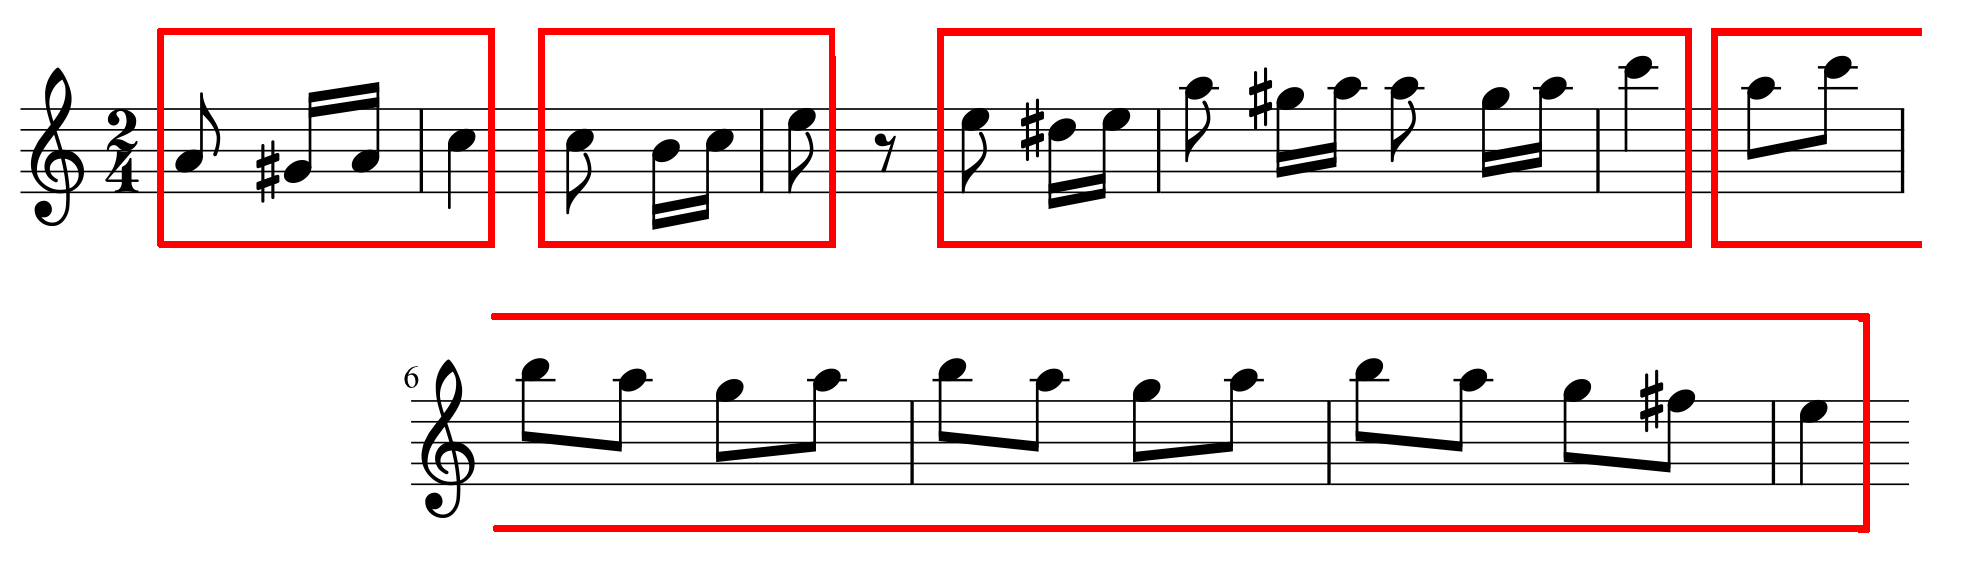
\includegraphics[scale=3]{img/melodysegments}
\caption{First four segments of piano sonata KV331 III by Mozart (grace notes are not shown)}
\end{figure}

NOTE (SECOND ORDER PITCH INTERVAL AND "SMOOTHED" IOI TREES FIGURES plus DISCUSSION)

The pitch interval segmentations are less reliable than the IOI segmentations but since we use pitch only to subdivide IOI segments we can still be sure that some constituent transitions are based on the more reliable IOI segmentation.

\subsection{Constituent Features}
\label{scorefeatures}

We can now convert a piece of music into a serie of constituents. These constituents will be used to predict expression so we must be able to charaterize them in a way correlates with the way they are performed. Analogous to YQX we are looking for the \textit{context} of the constituent as well as some description of the constituent itself.

YQX uses a set of three score features: pitch interval, duration ratio and I-R arch. The pitch interval is simply the difference in pitch between the current note and the next note. The duration ratio is the logarithmic ratio of the duration of the current note and the duration of the next note.  The I-R arch is is the distance to the nearest point of closure, where closure is calculated from the Implication-Realization analysis. NOTE(Too literally?)

We can generalize pitch interval and duration ratio per note to constituent features: \textit{mean pitch interval} and \textit{mean duration ratio}. Definitions can be found in table \ref{features}. Since I-R arch is related to note-level expression it does not generalize well to a constituent level feature. 

The two features above provide information about the constituent context: if they are both zero the constituent is apparently similar in mean pitch and mean duration. At note level there is not much to say about the current note besides the pitch and duration. However at constituent we would also like to say something about the constituent itself. For this purpose \textit{mean delta pitch} and \textit{mean delta duration} are used. These features say something about the amount change in pitch and the amount of change in note duration.

The complete set of score features consists of two \textit{context features} and two \textit{constituent features}:
\begin{description}
\item[\textbf{Mean pitch interval}] 
The difference between the mean pitch of the current constituent and the mean pitch of the next constituent, zero if the current is the last constituent
\item[\textbf{Mean duration ratio}]
The logarithmic ratio between the mean note duration of the current constituent and the mean note duration of the next constituent
\item[\textbf{Mean delta pitch}] The mean of all absolute pitch intervals within one constituent. 
\item[\textbf{Mean delta duration}] The mean of all absolute differences in duration of succeeding notes within one constituent
\end{description}

NOTE(Clearly, expressive markings in the score play a role in how the constituent should be played. If the segmentation is specific enough  there will hopefully be at most expressive marking within each constituent. )?

\subsection{Expression Parameters}
\label{targets}

Every constituent will be assigned expression parameters that indicate how the constituent is played expressively in a performance. These parameters define what we mean by structure level expression and should therefore be chosen carefully. 

Some concepts that we think fall under structure level expression are \textit{crescendo} or \textit{decrescendo}, \textit{ritardando} and \textit{piano} or \textit{forte} etc.
Concepts like crescendo, decrescendo and ritardando arguably fall under note level expression and for simplicity we will not consider them structure level expression. In fact, we will only look at the mean tempo, the mean articulation and the mean loudness of a constituent.

YQX defines expression per note in three parameters: \textit{IOI ratio}, \textit{articulation} and \textit{loudness}. These parameters are defined as the logarithmic ratio between the performance IOI and the IOI notated in the score (calculated using some base tempo), the silence after a score note divided by the silence after the performed note and the logarithmic ratio between the loudness of the performed note and the mean loudness of the performance. 

We are going to define our own expression parameters in a similar way but let us first look at some issues with the definitions YQX uses. The definition of articulations seems to be awkward and inconsistend. Awkward because if a score note is not followed by a rest, the notated silence after it is zero, rendering articulation undefined. Inconsisted because all the other features use logarithmic ratios and we see no reason to not use a logarithmic ratio for articulation as well. 

IOI ratio and loudness is defined relative to mean performance tempo and loudness. However, to capture micro expression in the form of small changes in onset relative to the beat, it seems more logical to define this feature relative to the local tempo, instead of relative to the global tempo. The same argument can be made for defining loudness relative to local loudness instead of global loudness. Structure level expression may help to define the concepts of local tempo and local loudness as we can simply take the mean tempo and loudness within one constituent and take this to be the local tempo and loudness.

The expression parameters that we will use are:
\begin{description}
\item[Mean Tempo Ratio] The logarithmic ratio between the mean tempo within the constituent and the base tempo of the performance.
\item[Mean Articulation] The logarithmic ratio between performance IOI and the score IOI if the next note is not a rest. If the next note is a rest we use the note duration calculated with the score duration of the note and the local expressive tempo instead of the performance IOI. IOI is the onset of the next note minus the onset of the current note.
\item[Mean Loudness Ratio] The logarithmic ratio of the mean loudness within the constituent and the base loudness of the performance
\end{description}

Admittedly, we still use mean loudness and tempo to calculate tempo and loudness ratio. This is a symptom of using a segmentation instead of hierarchical structure. When using hierarchical structure, these parameters could be defined relative to the parent constituent.

\subsection{Model}


We can now reduce a piece of music, represented as a sequence of notes $N_{ij}$, of which we have a score and a performance, to a sequence of score feature vectors $F$ and expression parameter vectors $E$. First, we segment the score into constituents:

\[\texttt{segment}(N_{ij}) = \{c_1, c_2, \cdots, c_n\}\]
We can then extract feature and parameter values from the score and the performance:
\begin{align*}
f_i &= (p_i, d_i, \Delta p_i, \Delta d_i)^T\\
F &= \{f_1, f_2, \cdots, f_n\}
\end{align*}
where $f_i$ is a feature vector, $p_i$ is the the mean pitch interval, $d_i$ is the mean duration ratio, $\Delta p_i$ is the mean delta pitch and $\Delta d_i$ is the mean delta duration.
And the expression parameters: 
\begin{align*}
e_i &= (t_i, a_i, l_i)^T\\
E &= \{e_1, e_2, \cdots, e_n\}
\end{align*}
where $e_i$ is a parameter vector, $t_i$ is the mean tempo ratio, $a_i$ is the mean articulation and $l_i$ is the mean loudness ratio.

If we parse a number of pieces is this manner we can use it to do some statistics. We can for example calculate the features likely-hood which is the conditional probability of a feature vector $f_i$ given an expression vector $e_i$.

\begin{equation}
\label{emission}
P(f_i|e_i) = \frac{c(f_i, e_i)}{c(e_i)}
\end{equation}

Where $c(x)$ is the number of occurences of $x$ in the corpus.
The expression transition probability is defined by
\begin{equation}
\label{transition}
P(e_i|e_{i-1}) = \frac{c(e_{i-1}, e_i)}{c(e_{i-1})}
\end{equation}
where we make the simplification that expression in one constituent is only dependend on the expression in the previous constituent which is of course not true.

The problem of creating a performance of a score is now reduced to finding a suitable sequence of expression vectors given a sequence of feature vectors. We can calculate the probability of one expression vector of a performance as the product the probabilities defined in equations \ref{emission} and \ref{transition}. The probability of the entire performance is approximated by the product of the individual expression vector probabilities.

\begin{equation}
P(E|F) = \displaystyle\prod_{i=1}^{n}P(f_i|e_i)P(e_i|e_{i-1})
\end{equation}

The resulting model is analogous to a stochastic part of speech tagger based on a hidden Markov model where we have substituted words for score feature vectors and parts of speech for expression parameter vectors. Rendering a performance is like finding the most likely part of speech tags for a sequence of words. In our case:

\[E^* = \texttt{argmax}_E P(E|F)\]

which can be found using Viterbi decoding.

\section{Implementation}


\begin{itemize}
\item Extract melody
\item Extract scorefeatures from melody
\item lookup notes in deviation, ignore missing notes
\item Extract expressive and non-expressive melody and extract expression features
\item Perform notes other than melody notes the same as the nearest melody note
\end{itemize}
\subsection{Corpus and Representation}
We were lucky to find and receive permission to use the CrestMusePEDB \ref{crestmuse} corpus, which is a corpus that contains expressive performances of Western classical music by famous pianists. The music includes works by Bach, Beethoven and Chopin.

Every performance is accompanied by an XML file containing information on how every note from the score is performed. This information consists of a loudness deviation, attack deviation and release deviation. The loudness is defined relative to a base loudness. The attack and release deviation are defined as the portion of a local beat duration that the attack and release deviates from the score. 

Local tempo is defined for every beat in every measure as the ratio of the tempo in that beat and the base tempo. 

To prepare a score and performance from the corpus for use in our system we use the score to extract melody notes. We do this simply by taking notes in the highest voice in the top staff. From now on when we talk about pieces and notes we mean melodies and melody notes.

Attack and release are clearly note level parameters so we do not use them. We only need tempo deviations and loudness deviations. The average tempo of a constituent is determined by the average tempo deviation of all the beats that fall within the constituent. The average loudness is determined by the average loudness deviation of every note within the constituent.

The deltafunctions that are used in the segmentation process use pitch intervals and duration ratios. The pitch intervals use MIDI note numbers which range from 21 to 108 and go up one semi-tone with each step. Durations are in milliseconds, calculated from the score and a standard tempo, set at 120 beats per minute.

\subsection{Discretization}
To calculate probabilities, we must discretize the feature and parameter vectors.

\paragraph*{Expression} Discretization of expression parameters is a delicate subject, we want to capture small changes in dynamics and tempo precisely, but outliers may fall in large bins. A sigmoid function is very useful for this purpose. The expression parameters are all logarithmic ratios so they theoretically vary from $-\infty$ to $\infty$. Therefore we first normalize the parameters by dividing through the mizimum absolute value found in the corpus. Discretization of a normalized expression parameter $p$ into $d$ bins is now done as follows:

\begin{equation}
D(p) = \texttt{floor}\left(\frac{d}{1+e^{-sp}}\right)
\end{equation}

Where $D(p)$ is the discretization of $p$, $s$ is a special sensitivity parameter indicating how small the changes in tempo that the discretization captures can be; a larger $s$ means a more sensitive discretization. Undiscretization is the reverse operation:

\begin{equation}
D^{-1}(p) = s^{-1} d^{-1}(-\log(p^{-1}) - 1)
\end{equation}

\paragraph*{Features}

To discretize the features, we simply normalize every feature dividing through the maximum absolute value of that feature found in the corpus. After normalization we multiply the feature by a discretization parameter $d$ that determines the number of bins and take the floor.

\begin{equation}
D(f) = \texttt{floor}(f*d)
\end{equation}

Where $f$ is the normalized feature value.

\subsection{Smoothing}

Despite having discretized our feature and observation vectors we often find that we observe feature vectors in a new score that we had never seen during training. We do not want the conditional probabilities from equation \ref{emission} to become zero so we have to smooth these probabilities. We use a smoothing technique known as simple Good-Turing smoothing. The idea is that we use the probabilities of things we have seen once for the things we have never seen. Recall how we calculate the conditional probability of a feature vector:
\[
P(f_i|e_i) = \frac{c(f_i, e_i)}{c(e_i)}
\]

Let us call the $c(f_i, e_i)$ the coincedence count. Let $N_c$ be the number of things with frequency $c$ in the corpus. For example if there are five coincedences $(f_x, e_x)$ nd no other pair of $f$ and $e$ occurs five times, then $N_{5} = 20$. Good-Turing re\"estimates counts according to this formula:

\begin{equation}
\label{count}
c^* = (c+1) \frac{N_{c+1}}{N_c}
\end{equation}

The smoothed probability of some event $x$ is

\[P(x) = \frac{c^*}{N}\]

In our case, the probability we seek is $P(f_i|e_i)$, the sample size $N$ is therefore the number of times we have seen $e_i$: $c(e_i)$. $N_c$ is the number of coincedences with $e_i$ that we have seen $c$ times. The count $c$ is $c(f_i, e_i)$ and $c^*$ is derived using equation \ref{count}. The 

\[P(f_i|e_i) = \frac{c^*}{c(e_i)} \mbox{ for all } c > 0 \]

By applying this formula to all counts larger than zero we reserve approximately $\frac{N_1}{N}$ probability mass for things that we have never seen. We assign an equal probability for all unseen feature vectors, namely:
\[
P(f_{\texttt{unseen}}|e_i) = \frac{1}{U} \frac{N_1}{c(e_i)} 
\]
Where U is the number of unseen coincedences, which is determined by the number of different observations in the corpus plus the new observations from the score minus the number of coincedences with $e_i$.

In order to make this work we cannot use $N_c$ directly since it will not be defined for every $c$. We use a least square apprixmation using the following function. 

\[\log(N_c) = a + b \log(c)\]

This completes the definition of simple Good-Turing smoothing. However, even now there may still be some expression parameter vectors that occur with unique feature vectors, so for that expression only $N_1$ is defined. We cannot fit a function to one sample, so if we have only one $Nc$ sample, we simply turn off Good-Turing smoothing and accept the fact that some probabilities will be zero. 

\subsection{Performance rendering}

Our model is able to generate expressively performed melodies but does not handle polyphony. During training, the bass and harmony notes were stripped off. After rendering an expressive performance we can simply put them back in and estimate their expressive parameters. We do this by this by by giving each  bass and harmony note the expressive parameters of the last played melody note. 

\begin{itemize}
\item Extract melody
\item Extract scorefeatures from melody
\item lookup notes in deviation, ignore missing notes
\item Extract expressive and non-expressive melody and extract expression features
\item Perform notes other than melody notes the same as the nearest melody note
\end{itemize}

\section{Evaluation and Results}

Using the method that we now have extensively described we have tried to generate a few performances of piano works by Mozart. The system was trained on 42 performances of 13 works by Mozart, see appendix \ref{appendix:corpus} for a more details. The choice for Mozart was motivated by the fact that our segmentation works best when phrase transitions are marked by long notes or silences, which is often the case in the work of Mozart. Another reason for choosing Mozart in favor of for example Chopin is that we think structure level expression is more outspoken in performances of Mozart's music.

%The system was tested on works from Mozart as we do not expect our system to generalize well to other composers.  We used

We discretized the score features using a discretization parameter of five. This means the constituent features (see section \ref{sec:features}) were discretized into five bins and the context features into a slightly larger number of bins since their values can be negative as well. The expression features where discretized into ten bins, with a sensitivity of five. These settings made sure we recognised most of the score features of a new score. The low number of bins does give the performances bit of a cartoonistic quality, but that does not make them any less interesting.




\subsection{Subjective Listening}
\subsection{Correlation}
\section{Integration with Note Level Performance Rendering}

The YQX system defines expressive tempo implicitly by predicting the logarithmic ratio of the IOI in a performance and the IOI in a score. Timing alterations of notes are always defined relative to the base tempo. This does not correspond to the intuition that the \textit{the tempo itself} is altered during the performance and that rhythmic changes should be seen relative to the local tempo. The same applies to the way YQX looks at loudness. This is specified as the logarithmic ratio between the notes loudness and the mean loudness of the performance. 

An intergration of constituent level expression and note level expression can provide a solution to this problem. We can define expressive tempo relative and dynamics relative to the expression parameters of the constituent

\section{Conclusion}
In this thesis we have critisized performance rendering systems that only use note level expression. 

We have introduced structure level expression and argued that a good performance rendering systems needs some notion of structure level expression. 

We have shown that we can create sensible segmentations of music based on an application of the delta framework. \cite{markwin} 

We have suggested a possible intergration of SBPR with note level performance rendering
\section{Discussion}

Unfortunately we do not have acces to the large dataset that YQX uses. The dataset we use is smaller. Since we do not learn per note but per group of notes, the impact of a smaller dataset is even larger. We have discretize into rather large bins for this reason, resulting in cartoonistic performances. 

We think we can afford to do this because:...

\begin{itemize}
\item Top notes is not always the melody, musical attention
\item Bass and harmony shouldn't be played with the same expression as melodynotes
\item Dataset size
\item Targets for expression level expression
\item Expressive markings
\item Staccato/articulation statistics
\item Backoff smoothing (doesn't assign equal probabilities to unseen events)
\end{itemize}

\section{Future Work}
\begin{itemize}
\item Combine deltatrees
\item Use loudness and tempo direction instead of means (requires more data)
\item Generalize approach to incorporate hierarchical structure, let structure extend to note level, so note level expression and structurelevel expression become integrated
\end{itemize}
\subsection{Repetition}
The system would certainly benefit from a notion of repetition and similarity. Repetition is a very good indicator of constituent breaks. Repetition and similarity could also be used to improve expressiveness of performances. It is probably telling when a phrase is repeated three times and then slightly altered the fourth time. Although finding similarity and musically significant repetition is a subject of its own the delta framework could help to define repetition arbitrarily of transposition or rhythm. A list of pitch deltas can for example be used to detect repetition independend of transposition and a list of duration deltas can be used to detect repetition of rhythm independend of the notes used. 

\section{Acknowledgements}

 \bibliographystyle{plain} % plain, nature, jbact
 \bibliography{myref} 

\appendix
\section{Corpus}
\label{appendix:corpus}
\begin{tabular}{ll}
\textbf{Work} & \textbf{Performer}\\
\hline
Sonata KV331 \MakeUppercase{\romannumeral 1}. & Hiroko Nakamura\\
& Glenn Gould\\
& Christoph Eschenbach\\
& Ingrid Haebler\\
& Lili Kraus\\
& Maria Jo\~ao Pires\\
& Alicia De Larrocha\\
& kn?\\
& yi?\\
& tn?\\
& Norio Shimizu\\
& mo\\
& mk?\\
& ea?\\
& nm?\\
& kt?\\
& tm?\\
\hline
Sonata KV331 \MakeUppercase{\romannumeral 2}. & Hiroko Nakamura\\
& Maria Jo\~ao Pires\\
& Alicia De Larrocha\\
& ea?\\
\hline
Sonata KV331 \MakeUppercase{\romannumeral 3}. & Hiroko Nakamura\\
& Maria Jo\~ao Pires\\
& Christoph Eschenbach\\
\hline
Sonata KV545 \MakeUppercase{\romannumeral 1}. & Maria Jo\~ao Pires\\
& Glenn Gould\\
\hline
Sonata KV545 \MakeUppercase{\romannumeral 2}. & Maria Jo\~ao Pires\\
& Glenn Gould\\
\hline
Sonata KV545 \MakeUppercase{\romannumeral 3}. & Maria Jo\~ao Pires\\
& Glenn Gould\\
\hline
Sonata KV279 \MakeUppercase{\romannumeral 1}. & Glenn Gould\\
& Maria Jo\~ao Pires\\
\hline
Sonata KV279 \MakeUppercase{\romannumeral 2}. & Glenn Gould\\
& Maria Jo\~ao Pires\\
\hline
Sonata KV279 \MakeUppercase{\romannumeral 3}. & Glenn Gould\\
& Maria Jo\~ao Pires\\
\hline
Sonata KV310 \MakeUppercase{\romannumeral 1}. & Maria Jo\~ao Pires\\
& Glenn Gould\\
& Hiroko Nakamura\\
Sonata KV310 \MakeUppercase{\romannumeral 2}. & Maria Jo\~ao Pires\\
Sonata KV310 \MakeUppercase{\romannumeral 3}. & Maria Jo\~ao Pires\\
Sonata KV570 \MakeUppercase{\romannumeral 3}. & nm?\\
\end{tabular}




 
 
\end{document}